\documentclass{standalone}
\usepackage{tikz}
\usetikzlibrary{patterns, positioning}


\begin{document}
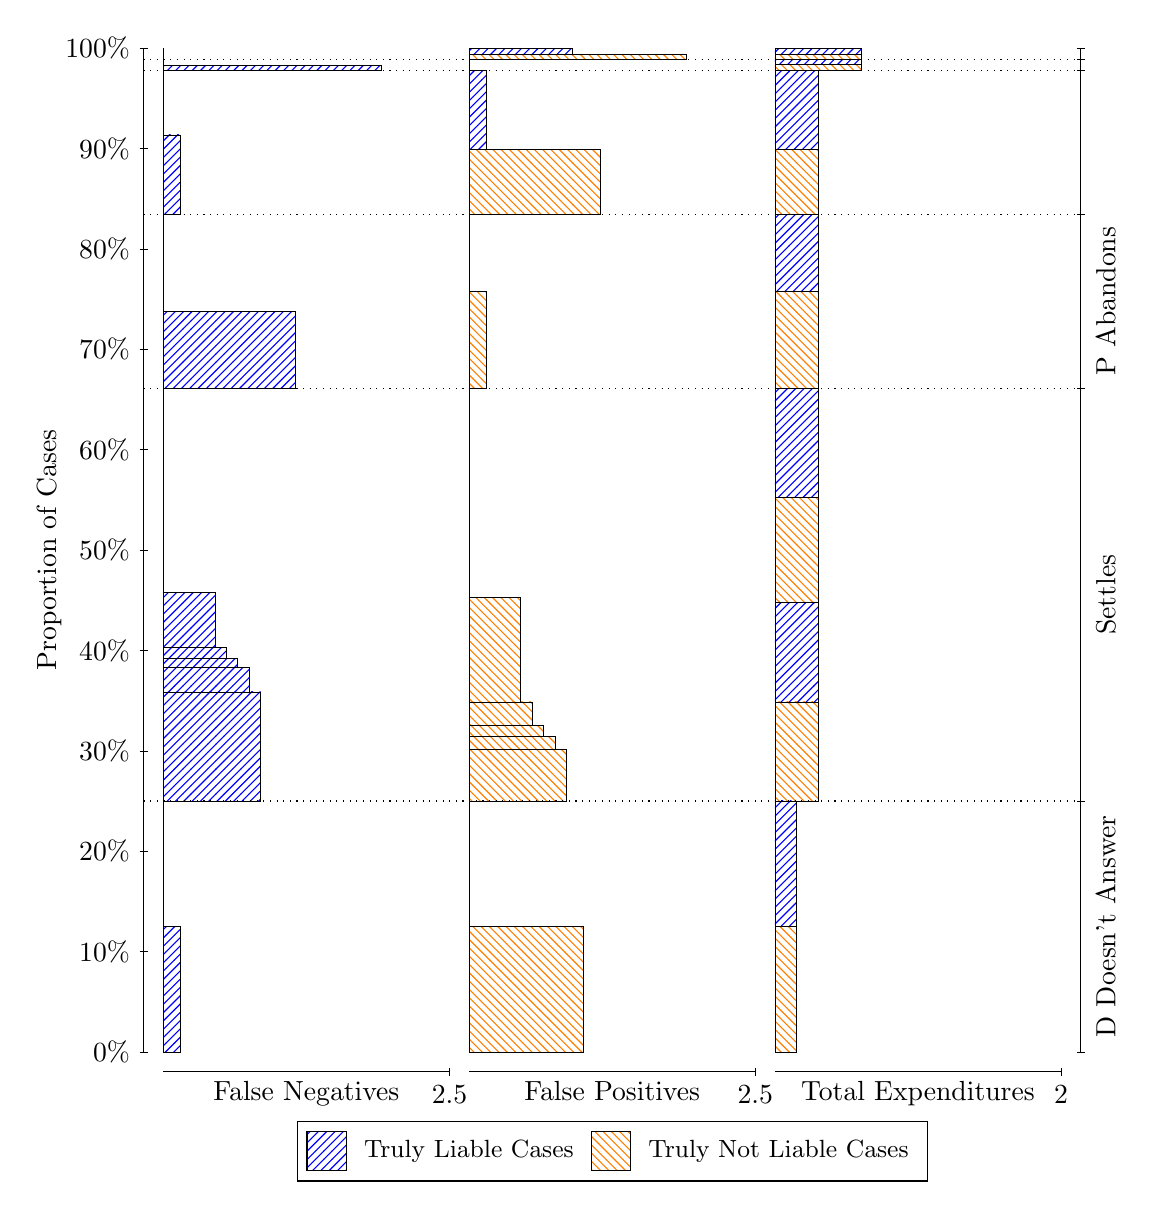
\begin{tikzpicture}
\draw[black, very thin] (1.5,1.75) -- (1.5,14.5);
\node[rotate=90, text=black, anchor=center] at (0.3, 8.125) {Proportion of Cases};
\draw[black, very thin] (1.45,1.75) -- (1.55,1.75);
\node[text=black, anchor=east] at (1.45, 1.75) {0\%};
\draw[black, very thin] (1.45,3.025) -- (1.55,3.025);
\node[text=black, anchor=east] at (1.45, 3.025) {10\%};
\draw[black, very thin] (1.45,4.3) -- (1.55,4.3);
\node[text=black, anchor=east] at (1.45, 4.3) {20\%};
\draw[black, very thin] (1.45,5.575) -- (1.55,5.575);
\node[text=black, anchor=east] at (1.45, 5.575) {30\%};
\draw[black, very thin] (1.45,6.85) -- (1.55,6.85);
\node[text=black, anchor=east] at (1.45, 6.85) {40\%};
\draw[black, very thin] (1.45,8.125) -- (1.55,8.125);
\node[text=black, anchor=east] at (1.45, 8.125) {50\%};
\draw[black, very thin] (1.45,9.4) -- (1.55,9.4);
\node[text=black, anchor=east] at (1.45, 9.4) {60\%};
\draw[black, very thin] (1.45,10.675) -- (1.55,10.675);
\node[text=black, anchor=east] at (1.45, 10.675) {70\%};
\draw[black, very thin] (1.45,11.95) -- (1.55,11.95);
\node[text=black, anchor=east] at (1.45, 11.95) {80\%};
\draw[black, very thin] (1.45,13.225) -- (1.55,13.225);
\node[text=black, anchor=east] at (1.45, 13.225) {90\%};
\draw[black, very thin] (1.45,14.5) -- (1.55,14.5);
\node[text=black, anchor=east] at (1.45, 14.5) {100\%};

\draw[black, very thin] (13.4,1.75) -- (13.4,14.5);
\draw[black, very thin] (13.35,1.75) -- (13.45,1.75);
\node[anchor=west] at (13.35, 1.75) {};
\draw[black, very thin] (13.35,4.9375) -- (13.45,4.9375);
\node[anchor=west] at (13.35, 4.9375) {};
\draw[black, very thin] (13.35,10.177) -- (13.45,10.177);
\node[anchor=west] at (13.35, 10.177) {};
\draw[black, very thin] (13.35,12.391) -- (13.45,12.391);
\node[anchor=west] at (13.35, 12.391) {};
\draw[black, very thin] (13.35,14.219) -- (13.45,14.219);
\node[anchor=west] at (13.35, 14.219) {};
\draw[black, very thin] (13.35,14.359) -- (13.45,14.359);
\node[anchor=west] at (13.35, 14.359) {};
\draw[black, very thin] (13.35,14.5) -- (13.45,14.5);
\node[anchor=west] at (13.35, 14.5) {};

\draw[black, very thin, pattern color=blue, pattern=north east lines] (1.75,1.75) rectangle (1.968,3.3437);
\draw[black, very thin, pattern color=orange, pattern=north west lines] (1.75,3.3437) rectangle (1.75,4.9375);
\draw[black, very thin, pattern color=blue, pattern=north east lines] (1.75,4.9375) rectangle (2.9853,6.3239);
\draw[black, very thin, pattern color=blue, pattern=north east lines] (1.75,6.3239) rectangle (2.84,6.6337);
\draw[black, very thin, pattern color=blue, pattern=north east lines] (1.75,6.6337) rectangle (2.6947,6.7507);
\draw[black, very thin, pattern color=blue, pattern=north east lines] (1.75,6.7507) rectangle (2.5493,6.8907);
\draw[black, very thin, pattern color=blue, pattern=north east lines] (1.75,6.8907) rectangle (2.404,7.5904);
\draw[black, very thin, pattern color=orange, pattern=north west lines] (1.75,7.5904) rectangle (1.75,10.177);
\draw[black, very thin, pattern color=blue, pattern=north east lines] (1.75,10.177) rectangle (3.4213,11.158);
\draw[black, very thin, pattern color=orange, pattern=north west lines] (1.75,11.158) rectangle (1.75,12.391);
\draw[black, very thin, pattern color=blue, pattern=north east lines] (1.75,12.391) rectangle (1.968,13.396);
\draw[black, very thin, pattern color=orange, pattern=north west lines] (1.75,13.396) rectangle (1.75,14.219);
\draw[black, very thin, pattern color=blue, pattern=north east lines] (1.75,14.219) rectangle (4.5113,14.284);
\draw[black, very thin, pattern color=orange, pattern=north west lines] (1.75,14.284) rectangle (1.75,14.359);
\draw[black, very thin, pattern color=orange, pattern=north west lines] (1.75,14.359) rectangle (1.75,14.424);
\draw[black, very thin, pattern color=blue, pattern=north east lines] (1.75,14.424) rectangle (1.75,14.5);
\draw[black, very thin, pattern color=orange, pattern=north west lines] (5.6333,1.75) rectangle (7.0867,3.3438);
\draw[black, very thin, pattern color=blue, pattern=north east lines] (5.6333,3.3438) rectangle (5.6333,4.9375);
\draw[black, very thin, pattern color=orange, pattern=north west lines] (5.6333,4.9375) rectangle (6.8687,5.5953);
\draw[black, very thin, pattern color=orange, pattern=north west lines] (5.6333,5.5953) rectangle (6.7233,5.7618);
\draw[black, very thin, pattern color=orange, pattern=north west lines] (5.6333,5.7618) rectangle (6.578,5.8951);
\draw[black, very thin, pattern color=orange, pattern=north west lines] (5.6333,5.8951) rectangle (6.4327,6.1952);
\draw[black, very thin, pattern color=orange, pattern=north west lines] (5.6333,6.1952) rectangle (6.2873,7.5237);
\draw[black, very thin, pattern color=blue, pattern=north east lines] (5.6333,7.5237) rectangle (5.6333,10.177);
\draw[black, very thin, pattern color=orange, pattern=north west lines] (5.6333,10.177) rectangle (5.8513,11.409);
\draw[black, very thin, pattern color=blue, pattern=north east lines] (5.6333,11.409) rectangle (5.6333,12.391);
\draw[black, very thin, pattern color=orange, pattern=north west lines] (5.6333,12.391) rectangle (7.3047,13.213);
\draw[black, very thin, pattern color=blue, pattern=north east lines] (5.6333,13.213) rectangle (5.8513,14.219);
\draw[black, very thin, pattern color=orange, pattern=north west lines] (5.6333,14.219) rectangle (5.6333,14.294);
\draw[black, very thin, pattern color=blue, pattern=north east lines] (5.6333,14.294) rectangle (5.6333,14.359);
\draw[black, very thin, pattern color=orange, pattern=north west lines] (5.6333,14.359) rectangle (8.3947,14.424);
\draw[black, very thin, pattern color=blue, pattern=north east lines] (5.6333,14.424) rectangle (6.9413,14.5);
\draw[black, very thin, pattern color=orange, pattern=north west lines] (9.5167,1.75) rectangle (9.7892,3.3438);
\draw[black, very thin, pattern color=blue, pattern=north east lines] (9.5167,3.3438) rectangle (9.7892,4.9375);
\draw[black, very thin, pattern color=orange, pattern=north west lines] (9.5167,4.9375) rectangle (10.062,6.1952);
\draw[black, very thin, pattern color=blue, pattern=north east lines] (9.5167,6.1952) rectangle (10.062,7.4617);
\draw[black, very thin, pattern color=orange, pattern=north west lines] (9.5167,7.4617) rectangle (10.062,8.7902);
\draw[black, very thin, pattern color=blue, pattern=north east lines] (9.5167,8.7902) rectangle (10.062,10.177);
\draw[black, very thin, pattern color=orange, pattern=north west lines] (9.5167,10.177) rectangle (10.062,11.409);
\draw[black, very thin, pattern color=blue, pattern=north east lines] (9.5167,11.409) rectangle (10.062,12.391);
\draw[black, very thin, pattern color=orange, pattern=north west lines] (9.5167,12.391) rectangle (10.062,13.213);
\draw[black, very thin, pattern color=blue, pattern=north east lines] (9.5167,13.213) rectangle (10.062,14.219);
\draw[black, very thin, pattern color=orange, pattern=north west lines] (9.5167,14.219) rectangle (10.607,14.294);
\draw[black, very thin, pattern color=blue, pattern=north east lines] (9.5167,14.294) rectangle (10.607,14.359);
\draw[black, very thin, pattern color=orange, pattern=north west lines] (9.5167,14.359) rectangle (10.607,14.424);
\draw[black, very thin, pattern color=blue, pattern=north east lines] (9.5167,14.424) rectangle (10.607,14.5);
\draw[black, dotted] (1.5,4.9375) -- (13.4,4.9375);
\draw[black, dotted] (1.5,10.177) -- (13.4,10.177);
\draw[black, dotted] (1.5,12.391) -- (13.4,12.391);
\draw[black, dotted] (1.5,14.219) -- (13.4,14.219);
\draw[black, dotted] (1.5,14.359) -- (13.4,14.359);
\draw[black, very thin] (1.75,1.5) -- (5.3833,1.5);
\node[text=black, anchor=north] at (3.5667, 1.5) {False Negatives};
\draw[black, very thin] (5.3833,1.45) -- (5.3833,1.55);
\node[text=black, anchor=north] at (5.3833, 1.45) {2.5};

\draw[black, very thin] (5.6333,1.5) -- (9.2667,1.5);
\node[text=black, anchor=north] at (7.45, 1.5) {False Positives};
\draw[black, very thin] (9.2667,1.45) -- (9.2667,1.55);
\node[text=black, anchor=north] at (9.2667, 1.45) {2.5};

\draw[black, very thin] (9.5167,1.5) -- (13.15,1.5);
\node[text=black, anchor=north] at (11.333, 1.5) {Total Expenditures};
\draw[black, very thin] (13.15,1.45) -- (13.15,1.55);
\node[text=black, anchor=north] at (13.15, 1.45) {2};

\node[text=black, centered, rotate=90] at (13.72, 3.3438) {D Doesn't Answer};
\node[text=black, centered, rotate=90] at (13.72, 7.5571) {Settles};
\node[text=black, centered, rotate=90] at (13.72, 11.284) {P Abandons};




\draw (7.449999999999999,1.5) node[draw=none] (baseCoordinate) {};
\begin{scope}[align=center]
        \matrix[scale=0.5, draw=black, below=0.5cm of baseCoordinate, nodes={draw}, column sep=0.1cm]{
            \node[rectangle, draw, minimum width=0.5cm, minimum height=0.5cm, pattern color=blue, pattern=north east lines] {}; &
            \node[draw=none, font=\small, text=black] (B) {Truly Liable Cases}; &
            \node[rectangle, draw, minimum width=0.5cm, minimum height=0.5cm, pattern color=orange, pattern=north west lines] {}; &
            \node[draw=none, font=\small, text=black] (B) {Truly Not Liable Cases}; \\
            };
\end{scope}

\end{tikzpicture}
\end{document}